%%==================================================
%% chapter03.tex for SJTU Bachelor Thesis
%% version: 0.5.2
%% Encoding: UTF-8
%%==================================================

% \bibliographystyle{sjtu2} %[此处用于每章都生产参考文献]

\chapter{控制与智能避障算法}
\label{chap:algorithm}

在本章将主要介绍模块化移动机器人控制系统的软件系统。由于本移动机器人具有自主移动,自主定位,自动避障,地图生成和最优路径计算等功能,所以需要将其软件系统分为底盘电机驱动,车体定位,未知环境避障和探测地图绘制等部分。其中只有电机驱动部分是与选用的控制芯片有关系的,而其他诸部分皆是上层算法,所以处理驱动算法的程序不可移植外,其他部分皆可移植到其他系统中去。在下面的介绍中,除了会给出具体算法程序外,还会对每一部分算法的数学原理进行简单的介绍,以期算法可以被很好地理解。

\section{底盘驱动算法}
底盘驱动采用了经典的H桥方案,通过单一IO口的高低电平来对方向进行控制,而在使能端接入PWM方波,通过控制占空比来控制电机的转速。控制占空比来控制转速的具体原理是,占空比的改变可以改变方波的等效电压。设一列方波的占空比是$a$,则在一个方波周期内等效电压与占空比的关系为 \\
\begin{equation}\label{eqn.equavalentVoltage}
V_{org}aT=V_{equ}T
\end{equation}
其中$V_{org}$是方波最大幅值,$T$为方波周期,$V_{equ}$为等效电压。通过公式\eqref{eqn.equavalentVoltage},可以得到\\
\begin{equation}
V_{equ} = aV_{org}
\end{equation}
等效电压与占空比呈简单线性关系。而通过电机的特性公式\eqref{eqn.motorCha} \\
\begin{equation}\label{eqn.motorCha}
V_{supply} = K_{e}\dot{\theta}
\end{equation}
可知电机转速和输入电压$V_{sipply}$成正比,这就意味轮子的转速与方波占空比成正比。所以控制轮子的转速只需要改变输入方波的占空比就可以了。但是占空比只给出了一个速度的相对关系,并没有与具体速度值的对应,所以控制的时候还要通过传感器的数据,对速度控制进行闭环。

电机系统所需输出口初始化,和一般电机控制程序如下。

在底盘模块正常情况下是沿着算法所确定的方向匀速行进,速度只需规定一个为常数的占空比值就可以了。但是因为电机特性不一致的原因,即便规定同一PWM值,车体行进方向仍然可能偏离既定方向,所以要使底盘保持行进方向,就要对其行进角度进行闭环。这一功能的可以通过电子罗盘返回的数据来设计实现。这里将采用传统的PID算法来进行闭环程序的设计。PID系统的传递方程为的拉普拉斯形式可以写为 \\
\begin{equation}
G(s)= K_p+\frac{K_i}{s}+K_ds
\end{equation}
其中$K_p$,$K_i$和$K_d$为PID方法的参数,对于系统方程,输入量是实际角度与计算角度的差值,输出量是驱动左轮与驱动右轮PWM占空比的差值。因为系统实际是离散的,所以需要将系统方程从S域映射到离散系统的Z域,关于这个控制器的C程序就是根据这一思想设计的,其伪代码可以表示如下。
\begin{lstlisting}[language={C}, caption={PID控制器伪代码}]
double KP = 一个合理的值;
double KI = 一个合理的值;
double KD = 一个合理的值;
double Error = 0;			//实际角度与计算角度的偏差
static double ErrorHis = 0;	//对于角度偏差的记录
static double ErrorAcu = 0;	//偏差积分

Error = AngleActual - AngleCalculated;
ErrorAcu += Error ;
DutyCycleDiff = KP*Error + KD*(Error-ErrorHis) + Ki*ErrorAcu ;
ErrorHis = Error;
\end{lstlisting}
关于底盘模块行进方向角度的计算将在未知环境避障算法部分介绍,关于遇到避障时转向的控制也将在那部分章节介绍。
\section{车体定位方案}
车体定位方案将直接决定了底盘模块的行进轨迹,对于是否完成目标的判断和地图的绘制等功能的实现。为了获得机器人准确的位置,在本设计中,使底盘集成了多种传感器模块。这其中包括轮式编码器,俗称拖地轮;IMU模块等单元,如果需要,则可以通过串口扩展,很容易的链接GPS模块。在下文中将详细介绍各个方案定位的数学原理,及坐标值获得的方法。

\subsection{拖地轮及方位角传感器定位}
拖地轮的机械结构设计已经在第二章的相应部分进行详细的叙述,在本节,将主要介绍基于拖地轮的定位算法。拖地轮的设计目标之一就要简化计算,所以将拖地轮固定在底盘模块相邻的两条边中央的位子上。底盘模块的坐标系,与轮子的位置如图\ref{fig.ChesisCoor} 所示。
\begin{figure}[!htp]
  \centering
  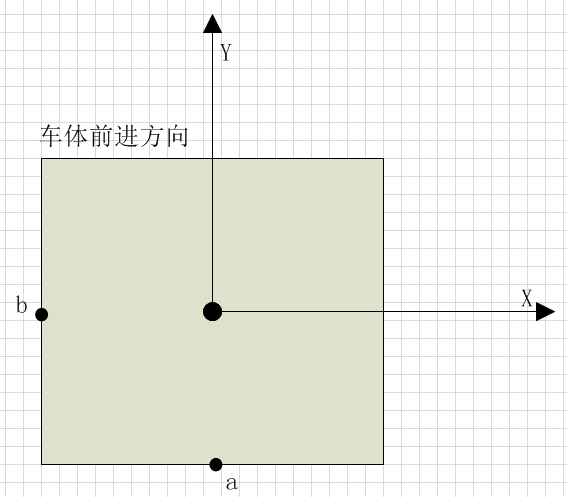
\includegraphics[width=0.5\textwidth]{chap4/ModelCordinates.PNG}
  \bicaption[fig.ChesisCoor]{底盘上坐标系的定义}{底盘上坐标系的定义}{Fig}{The Definition of the Coordinates On the Chassis}
\end{figure}

其中拖地轮a只能采集到与底盘模块y坐标轴平行的转动,同理拖地轮b只能采集到与底盘模块x坐标轴平行的转动。底盘的控制芯片将会以一定的周期进行对传感器信息的采集和对底盘模块体的控制。这一周期在本设计中为10毫秒,所以控制周期是100HZ。当每一个周期结束后,如果只有y方向的轮子采集到数据,则机器人体的世界坐标改变量为 \\
\begin{equation}
		\left\{
             \begin{array}{lcl}
            	\Delta x_{world} &= \Delta y\cdot \sin\theta \\
             	\Delta y_{world} &= \Delta y\cdot \cos\theta  
             \end{array}  
        \right.
\end{equation}
其中$x_{world}$,$y_{world}$为机器人体在世界坐标系中的坐标,$\theta$为机器人前进方向与世界坐标y轴所成的夹角。

同理当只有x方向的轮子采集到位移数据时,则机器人的世界坐标为 \\
\begin{equation}
		\left\{
             \begin{array}{lcl}
            	\Delta x_{world} &= \Delta x\cdot \cos\theta \\
             	\Delta y_{world} &= \Delta x\cdot \sin\theta  
             \end{array}  
        \right.
\end{equation}
而在同时采集到x与y方向的位移信息时,就需要用到一定的数学技巧来获得世界坐标的位移改变量。如图\ref{fig.ChesisMotion}所示,因为控制周期比较短,可以用直角模型来计算机器人体的位移,并假设车体的运动方向是初始时的运动方向保持不变,这样就可以通过机器人前进方向与世界坐标y轴的夹角和采集到的传感器信息来计算车体的实际位移了。
\begin{figure}[!htp]
  \centering
  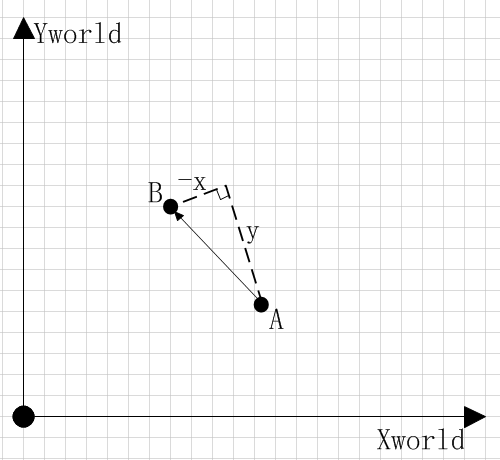
\includegraphics[width=0.5\textwidth]{chap4/OnMotion.PNG}
  \bicaption[fig.ChesisMotion]{机器人运动示意}{机器人运动示意}{Fig}{The Motion of the Robot in World Coordinates}
\end{figure}

这时世界坐标该变量的计算公式为 \\
\begin{equation}
		\left\{
             \begin{array}{lcl}
            	\Delta x_{world} &= \Delta y\cdot \sin\theta - \Delta x\cdot \cos\theta \\
             	\Delta y_{world} &= \Delta y\cdot \cos\theta + \Delta x\cdot \sin\theta  
             \end{array}  
        \right.
\end{equation}
\subsection{IMU定位}
通过IMU上所拥有的传感器元件可知,其对于位置的确定是依赖于积分的。加速度传感器的输出量是加速度,陀螺仪的输出量是角加速度,电子罗盘的输出量是角度。表征速度,位移和加速度关系的公式是 \\
\begin{equation}
D = \int\dot{D}=\int_T\int_T\ddot{D}
\end{equation}
所以只要对加速度进行二次积分就可以算出在某一轴上的位移分量。因为控制周期比较短,所以可以认为在一个周期内,机器人是在做匀加速度,匀速度运动。如果以$\ddot{x}$和$\ddot{y}$作为在底盘模块参考系中的加速度传感器所能测出的加速度量,则坐标的数学表达式可以写作 \\
\begin{equation}
		\left\{
             \begin{array}{lcl}
            	\Delta x_{world} &= \ddot{y}\cdot T^2\cdot \sin\theta - \ddot{x}\cdot T^2\cdot \cos\theta \\
             	\Delta y_{world} &= \ddot{y}\cdot T^2\cdot \cos\theta + \ddot{x}\cdot T^2\cdot \sin\theta  
             \end{array}  
        \right.
\end{equation}
但是因为加速度传感器的噪声带会对积分误差的收敛造成影响,所以光靠加速度传感器的值做计算是不够的。还需要加上陀螺仪的输出值作参考。加速度值与陀螺仪测得的关于垂直于地面平面的转轴的角加速度值的关系是 \\
\begin{equation}
\arctan(\frac{\ddot{x}\cdot T^2}{\ddot{y}\cdot T^2}) = \int_T\int_T \ddot{\phi}
\end{equation}
其中$\phi$是角加速度。

但是仅仅是使用这个比较依然是不可靠的,还要对采集到的数据进行滤波。本设计根据Houtekamer等人\upcite{houtekamer1998data} 的文章,设计了对信号处理的卡尔曼滤波器。其C程序实现如下。
\begin{lstlisting}[language={C}, caption={Kalman滤波的C程序代码}]
float angle, angle_dot; 		//外部需要引用的变量
float Q_angle = 0.05, Q_gyro = 0.01, R_angle = 5, dt = 0.005;     
float P[2][2] = {{ 1, 0 },{ 0, 1 }} ;	
float Pdot[4] ={0,0,0,0} ;
const char C_0 = 1;
float q_bias, angle_err, PCt_0, PCt_1, E, K_0, K_1, t_0, t_1;
//-------------------------------------------------------
void Kalman_Filter(float angle_m,float gyro_m)			
{
	angle+=(gyro_m-q_bias) * dt;			//先验估计
	
	Pdot[0]=Q_angle - P[0][1] - P[1][0];	//先验估计误差协方差的微分
	Pdot[1]=- P[1][1];
	Pdot[2]=- P[1][1];
	Pdot[3]=Q_gyro;
	
	P[0][0] += Pdot[0] * dt;				// 先验估计误差协方差
	P[0][1] += Pdot[1] * dt;
	P[1][0] += Pdot[2] * dt;
	P[1][1] += Pdot[3] * dt;
	
	
	angle_err = angle_m - angle;			
	
	PCt_0 = C_0 * P[0][0];
	PCt_1 = C_0 * P[1][0];
	
	E = R_angle + C_0 * PCt_0;
	
	K_0 = PCt_0 / E;//Kk
	K_1 = PCt_1 / E;
	
	t_0 = PCt_0;
	t_1 = C_0 * P[0][1];

	P[0][0] -= K_0 * t_0;					//后验估计误差协方差
	P[0][1] -= K_0 * t_1;
	P[1][0] -= K_1 * t_0;
	P[1][1] -= K_1 * t_1;
	
	angle	+= K_0 * angle_err;				//后验估计
	q_bias	+= K_1 * angle_err;				//后验估计
	angle_dot = gyro_m-q_bias;				//输出值(后验估计)的微分 = 角速度
}
\end{lstlisting}
\subsection{GPS定位}
因为GPS极差的室内信号的接收率,所以在本设计中并没有使用这一模块,不过作为常见的定位手段,在这里予以进行简单讨论。GPS模块往往为串口输出,输出遵从GPS标准协议,刷新频率为1Hz,即一秒输出一次。在本实验中这个输出频率显然太慢了。不过作为GPS模块,它会直接输出对象目标和运动方向角度。直接得到这些数据,是可以加快计算速度的,同时也使算法设计变得简单。不过GPS的另一个去点就是,民用级别的模块的精度极低,大概为5m,在地势复杂多变的环境中应用显然是不现实的。所以GPS模块更适合于户外开阔地势的定位使用。
\section{未知环境避障算法}

\section{地图生成和最优路径生成}
\section{本章小结}
